\section{Theorie}
\label{sec:Theorie}

Zunächst wird erklärt, wie grundsätzlich Röntgenstrahlung in einer Röntgenröhre entsteht.
tbd

\subsection{Entstehung von Röntgenstrahlung} \label{sec:Röntgenstrahlung}

\begin{figure}
    \begin{subfigure}{0.48\textwidth}
        \centering
        \includegraphics[width=\textwidth]{pictures/Aufbau_Rröhre.pdf}
        \caption{Schematische Darstellung einer Röntgenröhre. \cite{demtroeder2}}
        \label{fig:aufbau}
    \end{subfigure}
    \begin{subfigure}{0.48\textwidth}
        \centering
        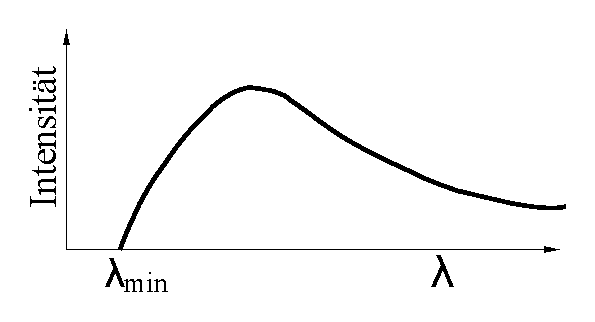
\includegraphics[width=\textwidth]{pictures/bremsspektrum.pdf}
        \caption{Das aufgrund von Energieabgabe kontinuierliche Bremsspektrum des Elektrons. \cite{v602}}
        \label{fig:bremsspektrum}
    \end{subfigure}
    \caption{Aufbau und kontinuierliches Spektrum einer Röntgenröhre.}
\end{figure}

Zur Erzeugung von Röntgenstrahlung werden in einer evakuierten Röhre aus einer Glühkathode
Elektronen emittiert und auf eine Anode hin beschleunigt.
Der schematische Aufbau einer Röntgenröhre ist in \autoref{fig:aufbau} dargestellt.
Die bei der Kollision austretende Strahlung besteht sowohl aus dem kontinuierlichen 
Bremsspektrum, dargestellt in \autoref{fig:bremsspektrum}, 
als auch aus der charakteristischen Röntgenstrahlung des Anodenmaterials.
Bei der Abbremsung eines Elektrons im Coulombfeld des Atomkerns werden Photonen emittiert, 
deren Energie dem Energieverlust den abgebremsten Elektronen entsprechen.
Die minimale Wellenlänge der Photonen bei vollständiger Abbremsung der Elektronen ergibt sich zu
\begin{equation}
    \lambda_\text{min} = \frac{h \cdot c}{e_0 \, U} \,
\end{equation}
wobei die gesamte kinetische Energie $E_\text{kin} = e_0 \, U$ in Strahlungsenergie umgewandelt wird.
Bei der charakteristischen Röntgenstrahlung wird durch Ionisation des Anodenmaterials ein Elektron in ein energetisch höheres Niveau versetzt oder ganz ausgelöst.
Fällt nun ein Elektron von einem energetisch höheren Zustand in ein niedrigeren, wird ein
ein Röntgenquant mit der Energie $h \, \nu = E_\text{m} - E_\text{n}$ emittiert. 
Dies entspricht der Energiedifferenz der beiden Energieniveaus, 
somit besitzt das Röntgenquant eine diskrete Energieverteilung die charakteristisch für das Anodenmaterial der Röntgenröhre.
Diese scharfen Linien werden mit $K_\alpha$, $K_\beta$, $L_\alpha$, ... bezeichnet, wobei $K$, $L$, $M$, ... die Schalen sind, auf denen die Übergänge enden.
Der griechische Buchstabe indexiert die Schale, aus der das Elektron stammt.

\subsection{Grundlagen zur Brechung}
\begin{figure}
    \centering
    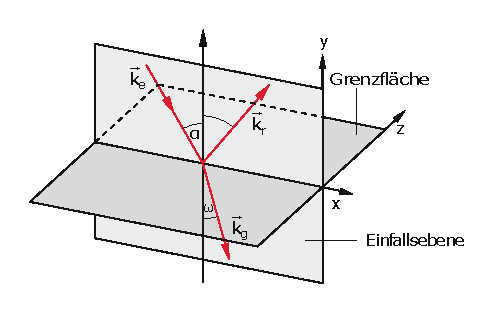
\includegraphics[width=0.6\textwidth]{pictures/Einfall.pdf}
    \caption{Einfall einer elektromagnetischen Welle auf eine Grenzfläche \cite{demtroeder2}.}
    \label{fig:einfall}
\end{figure}
Propagiert eine elektromagnetische Welle in ein anderes Medium, so kommt es zur Brechung.
Dies ist schematisch dargestellt in \autoref{fig:einfall}.
Die Brechung lässt sich durch den Brechungsindex
\begin{equation}
    n = 1 - \delta + i \beta
\end{equation}
beschreiben. Dabei ist $\delta$ ein Korrekturterm und $\beta$ die Absorption des Mediums.
Nun lässt sich mit dem Snelliusschen Brechungsgesetz
\begin{equation}
    \frac{n_1}{n_2} = \frac{\cos (\omega)}{\cos (\alpha)}
\end{equation}
und Vernachlässigung der Absorption die Formel für den kritischen Winkel herleiten, bei dem eine Totalreflexion auftritt.
Dafür setzt man voraus, dass $n_1 = n_\text{Luft} = 1$ ist.
Dann ergibt sich dür kleine $\delta$ \cite{tolan_xray}
\begin{equation}
    \alpha_C \approx \sqrt{2 \delta} = \lambda \sqrt{\frac{r_e \rho}{\pi}} \, .
\end{equation}
Dabei beschreibt $\rho$ die Elektronendichte im Medium und $r_e$ den klassischen Elektronenradius.

Des weiteren lässt sich mithilfe der Fresnelschen Formeln die Transmission und Reflexion von elektromagnetischen Wellen beschreiben.
Dabei lauten die Gleichungen
\begin{align*}
    r_s & =\frac{k_{i,z} - k_{t,z}}{k_{i,z} + k_{t,z}} \, ,\\
    r_p & =\frac{n^2 k_{i,z} - k_{t,z}}{n^2 k_{i,z} + k_{t,z}} \, ,\\
    t_s & =\frac{2 k_{i,z}}{k_{i,z} + k_{t,z}} \, ,\\
    t_p & =\frac{2 k_{i,z}}{n^2 k_{i,z} + k_{t,z}} \, .
\end{align*}
Dabei gilt $k_{i,z} = |k| \sin \alpha_i$ und $k_{t,z} = n |k| \sin \alpha_t$.
Da bei Röntgenstrahlung $n \approx 1$ ist, gilt $r_s = r_p$ und $t_s = t_p$.
Hieraus lässt sich dann der Fresnelsche Reflexionskoeffizient bestimmen.
Dieser ist bei $\alpha_i > 3 \alpha_C$ näherungsweise gegeben als \cite{tolan_xray}
\begin{equation}
    R\approx \left( \frac{\alpha_C}{2 \alpha_i} \right)^4 \, .
\end{equation}

\subsection{Reflektivität an Multischichtsystemen}
\begin{figure}
    \centering
    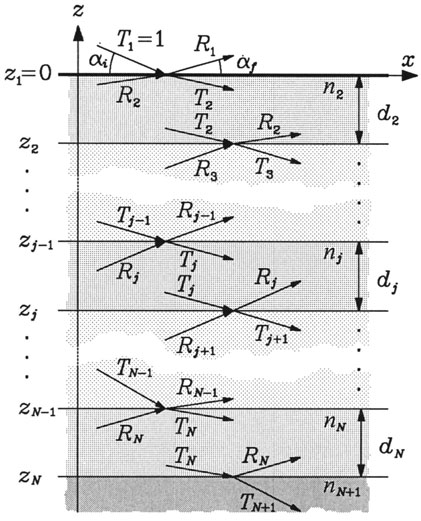
\includegraphics[width=0.6\textwidth]{pictures/multischicht.pdf}
    \caption{Darstellung einer mehrfachreflexion an einer Multischicht \cite{tolan_xray}.}
    \label{fig:multischicht}
\end{figure}